\section{Algoritmus 1}
\subsection{Zhrnutie algoritmu}
Algoritmus je písaný v programovacom jazyku \textit{Python}. Využíva knižnicu \textit{bpy 3.5.0}, ktorá pracuje s \textit{Blender}om. \textit{Blender} je program používaný na modelovanie 3D objektov. Algoritmus sa dá zhrnúť v nasledovných bodoch:
\begin{enumerate}
    \item Kontrola, či zadaný reťazec nie je veľkosťou viac ako 2**100
    \item Vytvorenie kociek
    \item Výpočet koordinácii jednotlivých bitov na veľkej kocke
    \item Prevod vstupného reťazca na binárny 
    \item Vyrezanie jednotlivých bitov
    \item Zmazanie malej kocky
    \item Zmena veľkosti veľkej kocky na požadovanú
\end{enumerate}


\subsection{Podrobný popis algoritmu}
V tejto podsekcií sú popísané jednotlivé body z predchádzajúcej sekcie spolu s útržkami kódu.

\subsubsection{Kontrola, či zadaný reťazec nie je veľkosťou viac ako 2**100}
V prípade porušenia podmienky algoritmus iba vypíše chybovú hlášku.
\\Kód:
\begin{lstlisting}[language=Python]
if (number > 2**100):
    raise ValueError("Number to encode can't be higher than 2^100.")
\end{lstlisting}

\subsubsection{Vytvorenie kociek}
Pri otvorení .blend súboru máme v projekte pridanú predpripravenú kocku so zrezanou hranou. Má zrezanú hranu, pretože 3D tlač nepodporuje tlačenie "do luftu". Preto sme pridali podpery pre kocky ktorými vyrezávame, aby sa identifikátor dal vytlačiť. Predpripravená kocka má uhol zrezania 14°. Ďalej programaticky vytvoríme veľkú a malú kocku. Do veľkej kocky budeme vyrezávať malou kockou a predpripravenou kockou. V podstate by sme programaticky vygenerovanú malú kocku nepotrebovali, ale na vrchu veľkej kocky nemusia byť žiadne podpery, preto vyrezávame celou kockou. \\Vytvorenie kociek: 
\begin{lstlisting}[language=Python]
    bpy.ops.mesh.primitive_cube_add(
        size=12, enter_editmode=False, align='WORLD', location=(0, 0, 0))
    bpy.context.active_object.name = 'big_cube'
\end{lstlisting}

\subsubsection{Výpočet koordinácii jednotlivých bitov na veľkej kocke}
Vstupom do funkcií je veľkosť veľkej kocky, veľkosť malej kocky a veľkosť výplne medzi bitmi.\\
Výpočet súradníc pre vrch kocky:
\begin{lstlisting}[language=Python]
def generate_ceil_coordinates(big_cube_size, small_cube_size, padding):
    wall_start = big_cube_size/2 - small_cube_size/2
    wall_start_with_padding = wall_start - padding

    z_current = wall_start
    z1_start = (-wall_start_with_padding, wall_start_with_padding)
    z1_array = []

    for i in range(10):
        for j in range(10):
            z1_array.append((round(z1_start[0] + j*small_cube_size, 3),
                            round(z1_start[1] - i*small_cube_size, 3), z_current))

    return z1_array
\end{lstlisting}
Výpočet súradníc pre boky kocky:
\begin{lstlisting}[language=Python]
def generate_wall_coordinates(big_cube_size, small_cube_size, padding):
    wall_start = big_cube_size/2 - small_cube_size/2
    wall_start_with_padding = wall_start - padding

    z_current = wall_start_with_padding
    x1_start = (wall_start, -wall_start_with_padding)
    x2_start = (-wall_start, wall_start_with_padding)
    y1_start = (wall_start_with_padding, wall_start)
    y2_start = (-wall_start_with_padding, -wall_start)

    x1_array = []
    x2_array = []
    y1_array = []
    y2_array = []

    for _ in range(10):
        for j in range(10):
            x1_array.append(
                (x1_start[0], round(x1_start[1] + j*small_cube_size, 3), z_current))
            x2_array.append(
                (x2_start[0], round(x2_start[1] - j*small_cube_size, 3), z_current))
            y1_array.append(
                (round(y1_start[0] - j*small_cube_size, 3), y1_start[1], z_current))
            y2_array.append(
                (round(y2_start[0] + j*small_cube_size, 3), y2_start[1], z_current))

        z_current = round(z_current - small_cube_size, 3)

    return [x1_array, x2_array, y1_array, y2_array]

\end{lstlisting}

\subsubsection{Prevod vstupného reťazca na binárny}
Vstupom do funkcie je číslo (menšie ako 2**100). Každá cifra z binárneho čísla sa prekonvertuje na binárnu hodnotu. Pre lepšie zobrazenie na kocke je binárne číslo obrátené a pre lepšie ladenie kódu doplnené o nuly na konci. Binárne číslo je obrátené, nuly by boli na začiatku takže by neovplyvnili hodnotu vstupného reťazca. \\Funkcia:
\begin{lstlisting}[language=Python]
def decimal_to_reversed_binary_list(number):
    reversed_binary_list = [int(x) for x in bin(number)[2:]]
    reversed_binary_list.reverse()
    while len(reversed_binary_list) != 100:
        reversed_binary_list.append(0)
    return reversed_binary_list
\end{lstlisting}
\subsubsection{Vyrezanie jednotlivých bitov}
Súradnice bitov na vrchu kocky sú pridané do poľa spolu so súradnicami bitov na kraji kocky.
\begin{lstlisting}[language=Python]
walls = generate_wall_coordinates(12, 1, 1)
ceil = generate_ceil_coordinates(12, 1, 1)
walls.append(ceil)
\end{lstlisting}
Neskôr sa prechádza všetkými jednotlivými stenami po jednotlivých bitoch. Naša predpripravená kocka je uložená v premennej \textit{my\_cube} a malá kocka je uložená v premennej \textit{small\_cube}. Pri každej stene má \textit{my\_cube} inú rotáciu aby podpery boli správne. Na vrchu veľkej kocky podpery nie sú potrebné, preto sa vyrezáva \textit{small\_cube}. Pri každom bite sa nastavuje umiestnenie \textit{my\_cube} a \textit{small\_cube}. Ak je index väčší ako 9, kontrolujeme či bit pod momentálnym bitom je 1, aby sme vedeli či potrebujeme vyrezať plnou kockou alebo zrezanou. Týmto predídeme problému na obrázku \ref{fig:problem_podpier}.
\begin{lstlisting}[language=Python]
wall_face = 0
for wall in walls:
    if(wall_face == 0):
        my_cube.rotation_euler[2] = math.radians(0)
    if(wall_face == 1):
        my_cube.rotation_euler[2] = math.radians(180)
    if(wall_face == 2):
        my_cube.rotation_euler[2] = math.radians(90)
    if(wall_face == 3):
        my_cube.rotation_euler[2] = math.radians(270)
    if(wall_face == 4):
       my_cube = small_cube
            
    for index, coordinate in enumerate(wall):
        if index > len(binary_list)-1 or binary_list[index] == 0:
            small_cube.location = coordinate
            my_cube.location = coordinate
            if index > 9 and binary_list[index-10] == 1:
                carve_out_with_object(big_cube, my_cube)
            else:
                carve_out_with_object(big_cube, small_cube)
    wall_face = wall_face + 1
\end{lstlisting}
\begin{figure}[H]
    \centering
    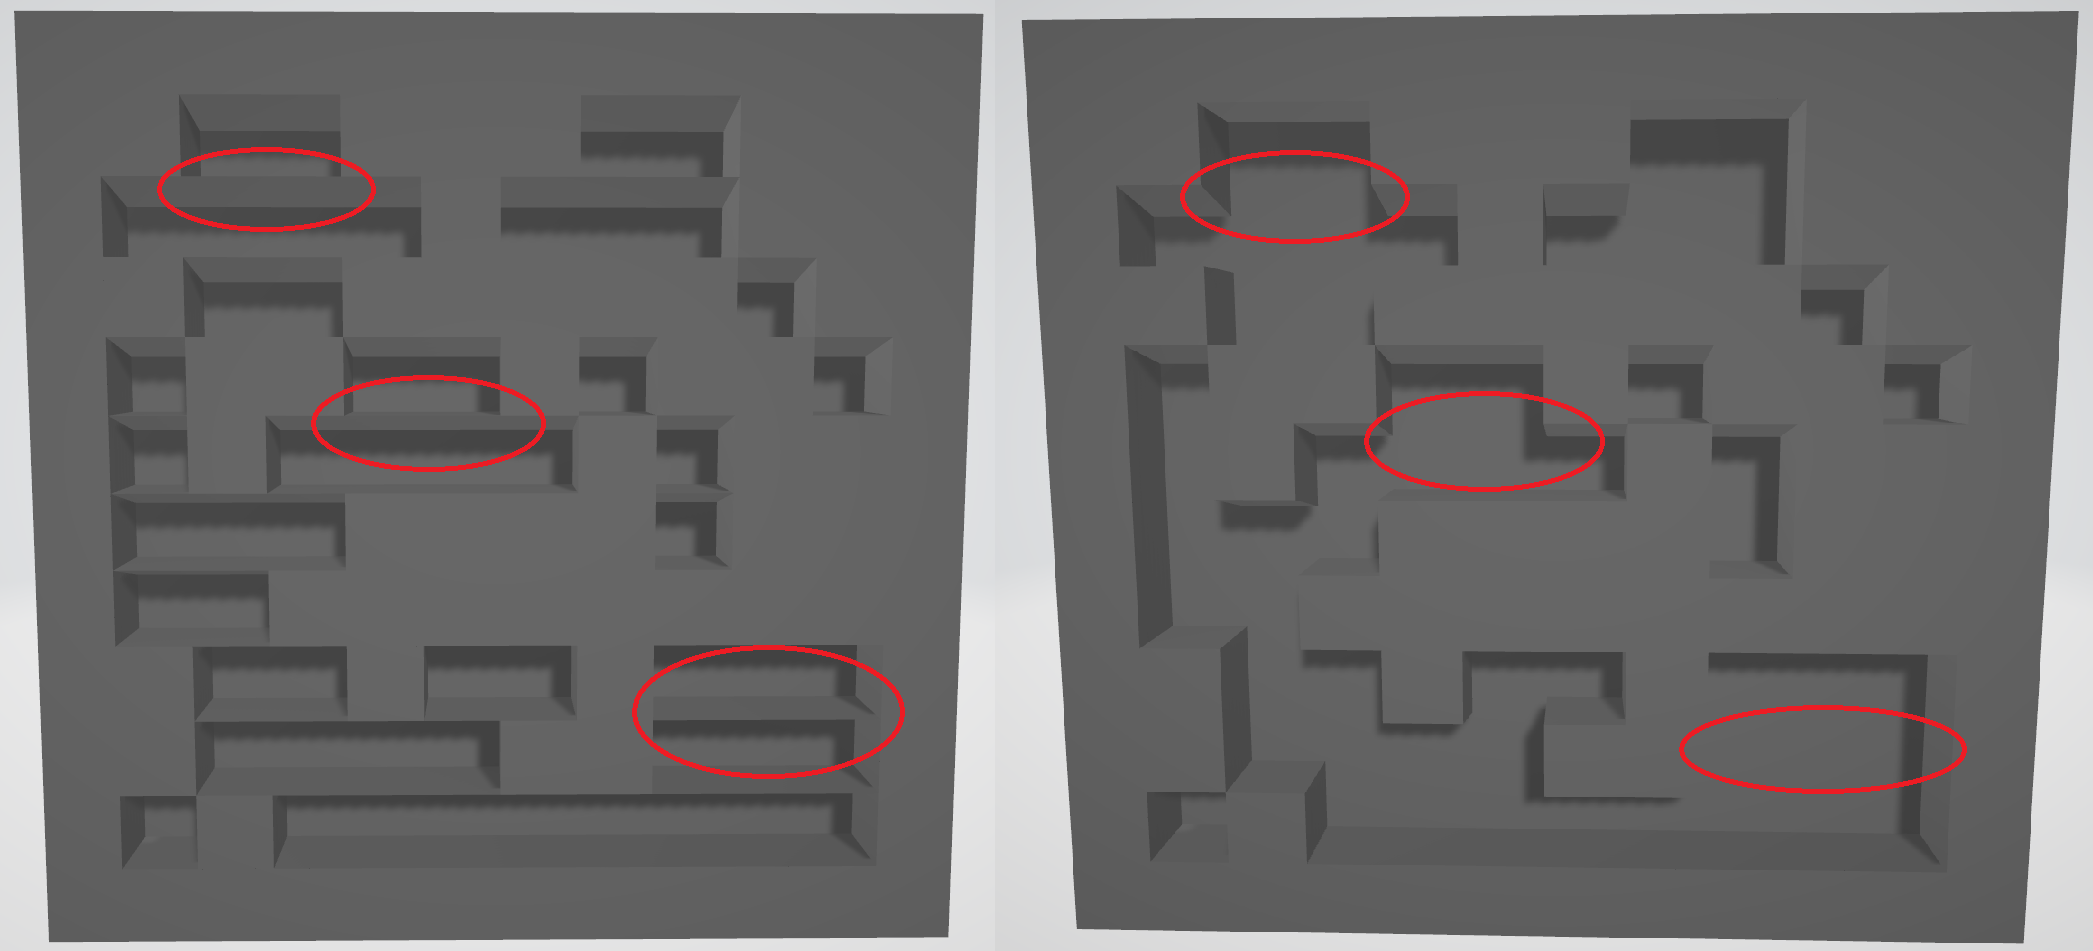
\includegraphics[scale=0.3]{includes/pictures/odstranenie_podpier.png}
    \captionof{figure}{Odstránenie zbytočných podpier}
    \label{fig:problem_podpier}
\end{figure}

\subsubsection{Zmazanie malej kocky}
Malú kocku odstránime, lebo ostáva na pozicií posledného vyrezávaného bitu a mohlo by sa stať, že načítame po vytlačení identifikátora iný reťazec.
\begin{lstlisting}[language=Python]
select_object(bpy.data.objects['cube'])
bpy.ops.object.delete()
select_object(bpy.data.objects['vyrez'])
bpy.ops.object.delete()
\end{lstlisting}

\subsubsection{Zmena veľkosti veľkej kocky na požadovanú}
Nakoniec zmenšíme kocku na požadovanú veľkosť pomocou príkazov:
\begin{lstlisting}[language=Python]
select_object(big_cube)
big_cube.dimensions = [wall_size_m, wall_size_m, wall_size_m]
\end{lstlisting}
